\documentclass{article}
\usepackage{cite}
\usepackage{amsmath,amssymb,amsfonts}
\usepackage{graphicx}
\newtheorem{theorem}{Theorem}
\newtheorem{lemma}{Lemma}
\newtheorem{definition}{Definition}
\newtheorem{note}{Note}
\newtheorem{property}{Property}

\newcommand{\fbf}{\mathbf{f}}
\newcommand{\Jbf}{\mathbf{J}}
\newcommand{\Mbf}{\mathbf{M}}
\newcommand{\mbf}{\mathbf{m}}
\newcommand{\pbf}{\mathbf{p}}
\newcommand{\ubf}{\mathbf{u}}
\newcommand{\vbf}{\mathbf{v}}
\newcommand{\deltabf}{\boldsymbol{\delta}}
\newcommand{\omegabf}{\boldsymbol{\omega}}
\newcommand{\taubf}{\boldsymbol{\tau}}


\title{Path Planning Challenge}
\author{Magicc Lab, Summer 2023}
\date{\today}

\begin{document}

\maketitle
\thispagestyle{empty}

    \begin{abstract}
        Convex optimization challenge for summer 2023.
    \end{abstract}

%-------------------------------------------------------
\section{Introduction}

The convex optimization challenge will use the VTOL example from~\cite{BeardMcLainPeterson}, which is describe below for convenience.  


\begin{figure}
  % Requires \usepackage{graphicx}
  \centering
  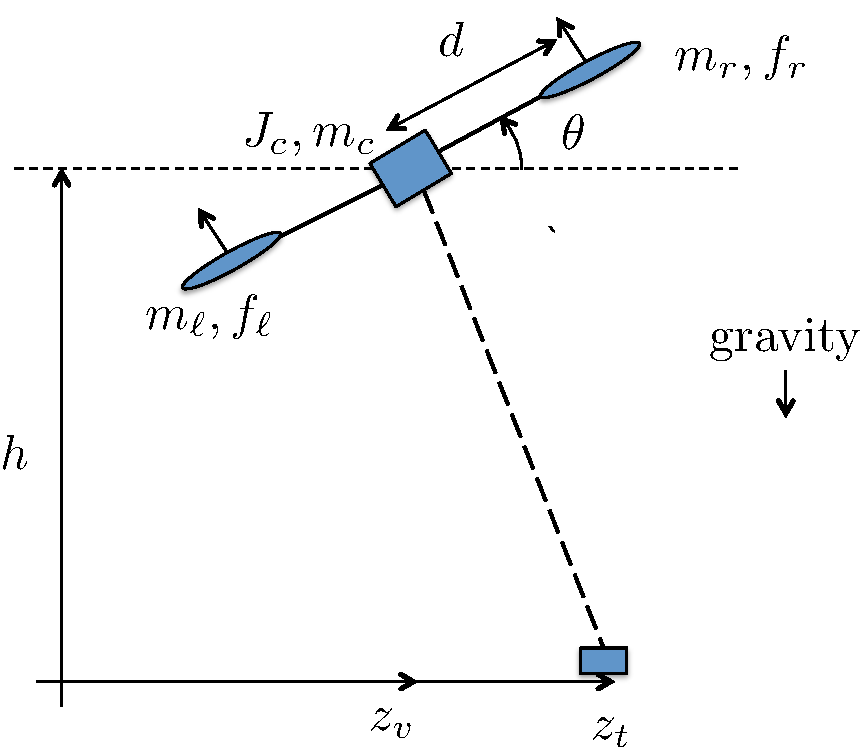
\includegraphics[width=0.59\textwidth]{figures/hw_planar_VTOL_defn}\\
  \caption{Planar vertical take-off and landing (VTOL)}
  \label{fig:planar_VTOL_defn}
\end{figure}

In this design study we will explore the control design for a simplified planar version of a quadrotor following a ground target.  In particular, we will constrain the dynamics to be in two a dimensional plane. In Cartesian space, the position of the VTOL can be defined by a variable describing the vertical position, one describing the horizontal position, and one angular variable describing the orientation, as shown in \ref{fig:planar_VTOL_defn}.  The planar vertical take-off and landing (VTOL) system is comprised of a center pod of mass $m_c$ and inertia $J_c$, a right motor/rotor that is modeled as a point mass $m_r$ that exerts a force $f_r$ at a distance $d$ from the center of mass, and a left motor/rotor that is modeled as a point mass $m_\ell$ that exerts a force $f_\ell$ at a distance $-d$ from the center of mass.  The position of the center of mass of the planar VTOL system is given by horizontal position $z_v$ and altitude $h$.  The airflow through the rotor creates a change in the direction of flow of air and causes what is called ``momentum drag.''  Momentum drag can be modeled as a viscous drag force that is proportional to the horizontal velocity $\dot{z}_v$.  In other words, the drag force is $F_{\text{drag}}=-\mu \dot{z}_v$.  The target on the ground will be modeled as an object with position $z_t$ and altitude $h=0$.  We will not explicitly model the dynamics of the target.  

Use the following physical parameters:
$m_c=1$~kg,
$J_c=0.0042$~kg m$^2$,
$m_r=0.25$~kg,
$m_\ell=0.25$~kg,
$d=0.3$~m,
$\mu = 0.1$~kg/s,
$g=9.81$~m/s$^2$.





%-------------------------------------------------------
\section{Dynamics}

The dynamics are given by
\begin{equation}\label{eq:vtol_sim_model}
\begin{pmatrix}
m_c + 2 m_r & 0           & 0 \\
0           & m_c + 2 m_r & 0 \\
0           & 0           & J_c + 2 m_r d^2
\end{pmatrix}
\begin{pmatrix}
\ddot{z} \\
\ddot{h} \\
\ddot{\theta}
\end{pmatrix}
=
\begin{pmatrix}
-(f_r + f_\ell) \sin\theta - \mu\dot{z} \\
-(m_c + 2 m_r) g + (f_r + f_\ell) \cos\theta \\
d \left( f_r - f_\ell \right)
\end{pmatrix}.
\end{equation}

We will assume that the right and left rotor forces are constrained as follows
\begin{equation}\label{eq:input_constraints}
	0\leq f_r, f_\ell \leq 0.75 (m_c + 2 m_r)g.
\end{equation}
If the thrust was limited to $0.5 (m_c + 2 m_r)g$, then at full throttle, the VTOL could just hover.  Therefore, the limit allows some additional control authority, but is somewhat constraining.


%-------------------------------------------------------
\section{Linearization}
Since $f_r$ and $f_\ell$ appear in the equations as either $f_r+f_\ell$ or $d(f_r-f_\ell)$, it is easier to think of the inputs as the total force $F\triangleq f_r+f_\ell$, and the torque $\tau\triangleq(f_r-f_\ell)$.  Note that since
\[
\begin{pmatrix} F \\ \tau \end{pmatrix} = \begin{pmatrix} 1 & 1 \\ d & -d \end{pmatrix}\begin{pmatrix} f_r \\ f_\ell \end{pmatrix},
\]
that
\[
\begin{pmatrix} f_r \\ f_\ell \end{pmatrix} = \begin{pmatrix} 1 & 1 \\ d & -d \end{pmatrix}^{-1}\begin{pmatrix} F \\ \tau \end{pmatrix}
= \begin{pmatrix} \frac{1}{2} & \frac{1}{2d} \\ \frac{1}{2} & -\frac{1}{2d} \end{pmatrix} \begin{pmatrix} F \\ \tau \end{pmatrix}.
\]
Therefore, 
\begin{align*}
f_r &= \frac{1}{2} F + \frac{1}{2d}\tau \\
f_\ell &= \frac{1}{2}F - \frac{1}{2d}\tau.
\end{align*}

Using the expression $F = f_r + f_l$ and $\tau = d (f_r - f_l)$, the equations of motion are given by
\begin{equation*}
\begin{pmatrix}
m_c + 2 m_r & 0           & 0 \\
0           & m_c + 2 m_r & 0 \\
0           & 0           & J_c + 2 m_r d^2
\end{pmatrix}
\begin{pmatrix}
\ddot{z} \\
\ddot{h} \\
\ddot{\theta}
\end{pmatrix}
=
\begin{pmatrix}
-F \sin\theta - \mu \dot{z} \\
-(m_c + 2 m_r) g + F \cos\theta \\
\tau
\end{pmatrix}.
\end{equation*}
At equilibria when $\dot{z} = \ddot{z} = \dot{h} = \ddot{h} = \dot{\theta} = \ddot{\theta} = 0$ we have
\begin{align}
- F_e \sin\theta_e &= 0 \label{Eq:VTOL_EqulibriumConstraint1} \\
- \left( m_c + 2 m_r\right) g + F_e\cos\theta_e &= 0 \label{Eq:VTOL_EqulibriumConstraint2} \\
\tau_e &= 0. \label{Eq:VTOL_EqulibriumConstraint3}
\end{align}
From Equation~\eqref{Eq:VTOL_EqulibriumConstraint1}, either $\theta_e = 0$ or $F_e = 0$, since $F_e = 0$ would make Equation~\eqref{Eq:VTOL_EqulibriumConstraint2} impossible to satisfy, we conclude that $\theta_e = 0$.
From \eqref{Eq:VTOL_EqulibriumConstraint1}, $F_e = \left(m_c + 2 m_r\right) g$, which makes sense since that is the force required to keep the VTOL in place.  

To linearize, define
\begin{align*}
\tilde{\theta} \triangleq \theta - \theta_e &\qquad \Rightarrow \qquad \theta = \theta_e + \tilde{\theta} \\
\tilde{F} \triangleq F - F_e &\qquad \Rightarrow \qquad F = F_e + \tilde{F}
\end{align*}
to get
Therefore, the linear equations of motion are
\begin{align*}
\left( m_c + 2 m_r \right) \ddot{\tilde{z}} + \mu \dot{\tilde{z}} &=  -F_e \tilde{\theta}   \\
\left( m_c + 2 m_r \right) \ddot{\tilde{h}} &= \tilde{F}\\
\left( J_c + 2 m_r d^2 \right) \ddot{\tilde{\theta}} &= \tilde{\tau}.
\end{align*}

Since the two nonlinearities are in the equations of motion cannot simultaneously be eliminated by correct choice of the single input $F$, feedback linearization is not a viable option for this system.


%-------------------------------------------------------
\section{State Space Equations}

Defining the state as
\[
x \triangleq \begin{pmatrix} z & h & \theta & \dot{z} & \dot{h} & \dot{\theta} \end{pmatrix}, 
\]
we get that
\[
\dot{x} = Ax + Bu
\]
where
\[
u = \begin{pmatrix} \tilde{F} \\ \tau \end{pmatrix}
\]
\begin{align*}
A &= \begin{pmatrix}
	0 & 0 & 0 & 1 & 0 & 0 \\
	0 & 0 & 0 & 0 & 1 & 0 \\
	0 & 0 & 0 & 0 & 0 & 1 \\
	0 & 0 & -\frac{F_e}{m_c+2m_r} & -\frac{\mu}{m_c+2m_r} & 0 & 0 \\
	0 & 0 & 0 & 0 & 0 & 0 \\
	0 & 0 & 0 & 0 & 0 & 0 
 	\end{pmatrix} \\
 B &= \begin{pmatrix}
 		0 & 0 \\
 		0 & 0 \\
 		0 & 0 \\
 		0 & 0 \\
 		\frac{1}{m_c+2m_r} & 0 \\
 		0 & \frac{1}{J_c+2m_rd^2}
 	  \end{pmatrix}
\end{align*}


%-------------------------------------------------------
\section{Trajectory Following}

Assume that the trajectory generator produces a reference trajectory $(x^r(t), u^r(t))$, and define the reference trajectory error as
\[
\tilde{x}\triangleq x - x^r, \qquad\qquad \tilde{u}\triangleq u-u^r,
\]
then
\begin{align*}
\dot{\tilde{x}} &= \dot{x} - \dot{x}^r \\
				&= Ax + Bu - \dot{x}^r + (Ax^r + Bu^r) - (Ax^r+Bu^r) \\
				&= A\tilde{x} + B\tilde{u} + (Ax^r + Bu^r - \dot{x}^r).
\end{align*}
Note that if the reference trajectory is {\em feasible} in the sense that the reference trajectory 
satisfies the dynamics, i.e., 
\[
\dot{x}^r = A x_r + B u^r,
\]
then
\[
\dot{\tilde{x}} = A\tilde{x} + B\tilde{u}.
\]
Otherwise, the term $d\triangleq Ax^r + Bu^r - \dot{x}^r$ can be thought of as a disturbance acting on the system.

Following the integrator design described in Chapter~12 of~\cite{BeardMcLainPeterson}, we desire to add integrators on position $z$ and altitude $h$.  Define
\[
C = \begin{pmatrix}
	1 & 0 & 0 & 0 & 0 & 0 \\
 	0 & 1 & 0 & 0 & 0 & 0
    \end{pmatrix}
\]
and the integrator state
\[
x_I = \int_{-\infty}^t C\tilde{x}(\tau)d\tau,
\]
which implies that
\[
\dot{x}_I = C\tilde{x},
\]
or 
\[
\frac{d}{dt}\begin{pmatrix}\tilde{x} \\ x_I \end{pmatrix} = \begin{pmatrix} A & 0 \\ C & 0 \end{pmatrix} \begin{pmatrix}\tilde{x} \\ x_I \end{pmatrix} + \begin{pmatrix} B \\ 0 \end{pmatrix}\tilde{u}.
\]
Defining
\[
A_1 \triangleq \begin{pmatrix} A & 0 \\ C & 0 \end{pmatrix}, 
\qquad
B_1 \triangleq \begin{pmatrix} B \\ 0 \end{pmatrix},
\qquad
K_1 \triangleq \begin{pmatrix} K & K_I \end{pmatrix},
\]
we find $K_1$ using {\tt K\_1 = place(A\_1, B\_1, p\_1)}, where $p_1$ are the desired poles.  The trajectory following controller is given by
\begin{align*}
	&\tilde{u} = - \begin{pmatrix} K & K_I \end{pmatrix} \begin{pmatrix}\tilde{x} \\ x_I \end{pmatrix} \\	
	\implies & \tilde{u} = -K\tilde{x} - K_I \int_{-\infty}^t C\tilde{x}(\tau)d\tau \\
	\implies & u = u^r - K(x-x^r) - K_I\int_{-\infty}^t C(x-x^r)d\tau \\
	\implies & \begin{pmatrix}F \\ \tau \end{pmatrix} = \begin{pmatrix}F_e \\ 0 \end{pmatrix} +  u^r - K(x-x^r) - K_I\int_{-\infty}^t C(x-x^r)d\tau \\
	\implies & \begin{pmatrix}f_\ell \\ f_r \end{pmatrix} = \begin{pmatrix}\frac{1}{2} & -\frac{1}{2d} \\ \frac{1}{2} & \frac{1}{2d} \end{pmatrix}\left[ \begin{pmatrix}F_e \\ 0 \end{pmatrix} +  u^r - K(x-x^r) - K_I\int_{-\infty}^t C(x-x^r)d\tau \right].
\end{align*}

%-------------------------------------------------------
\section{Landing Constraints}

The objective is to minimize the time $t_f$ required to land the VTOL from initial state
\[
x(t_0) = \begin{pmatrix}z(t_0) & h(t_0) & \theta(t_0) & \dot{z}(t_0) & \dot{h}(t_0) & \dot{\theta}(t_0) \end{pmatrix}^\top,
\]
to the final state
\[
x(t_f) = \begin{pmatrix} z(t_f) \\ h(t_f) \\ \theta(t_f) \\ \dot{z}(t_f) \\ \dot{h}(t_f) & \dot{\theta}(t_f) \end{pmatrix} 
	   = \begin{pmatrix} 0 \\ 0 \\ 0 \\ 0 \\ -0.1 & 0 \end{pmatrix}
\]
while satisfying the state constraints
\begin{align*}
	m_1^\top (C_c x - p_1) &\geq 0 \\
	m_2^\top (C_c x - p_2) &\geq 0,	
\end{align*}
where
\begin{align*}
C_c &= \begin{pmatrix} 1 & 0 & 0 & 0 & 0 & 0 \\ 0 & 1 & 0 & 0 & 0 & 0 \end{pmatrix} \\
m_1 &= \begin{pmatrix} \cos\varphi & \sin\varphi \end{pmatrix}^\top \\	
m_2 &= \begin{pmatrix} \cos\varphi & -\sin\varphi \end{pmatrix}^\top \\	
p_1 &= \begin{pmatrix} 0 & 0 \end{pmatrix}^\top \\	
p_2 &= \begin{pmatrix} 0 & 0 \end{pmatrix}^\top,
\end{align*}
where $\varphi = 30\pi/180$. 
The constraints are shown schematically in Figure~\ref{fig:constraints}.

The planned trajectory must also satisfy the input constraints given in Equation~\eqref{eq:input_constraints}.


\begin{figure}
  % Requires \usepackage{graphicx}
  \centering
  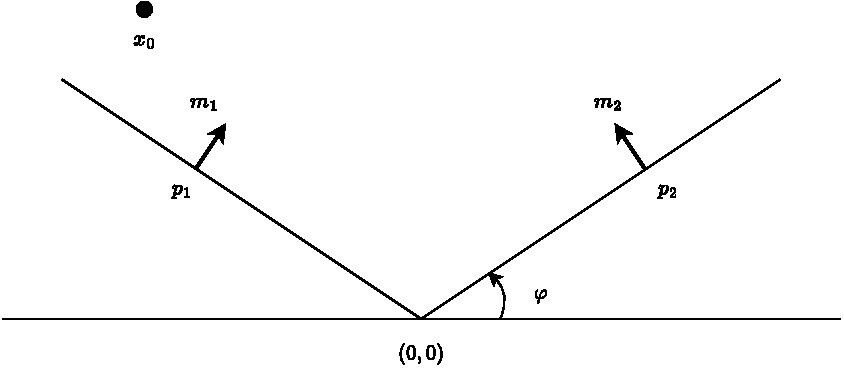
\includegraphics[width=0.59\textwidth]{figures/landing_constraints}\\
  \caption{State constraints}
  \label{fig:constraints}
\end{figure}


\bibliographystyle{IEEEtran}
\bibliography{library}

\end{document}

